%% ============================================================
%% main.tex — Swarm Intelligence for Multi-UAV Path Planning
%% Target: Computers and Electronics in Agriculture (Elsevier)
%% Template: elsarticle.cls (XeLaTeX)
%% Author: Andres Hidalgo Morales, Ph.D. Candidate
%% ORCID: 0000-0002-1074-9395
%% Instituto Tecnológico de Chihuahua II, TecNM
%% ============================================================

\documentclass[review, 12pt, times]{elsarticle}

%% ---- PACKAGES ----
\usepackage{lineno}
\usepackage{booktabs}
\usepackage{tabularx}
\usepackage{multirow}
\usepackage{graphicx}
\usepackage{hyperref}
\usepackage{xcolor}
\usepackage{amsmath}
\usepackage{longtable}
\usepackage{array}
\usepackage{pdflscape}
\usepackage[utf8]{inputenc}
\usepackage{fontspec}
\usepackage{tikz}
\usetikzlibrary{shapes, arrows.meta, positioning}

%% ---- LINE NUMBERS ----
\linenumbers

%% ---- JOURNAL ----
\journal{Computers and Electronics in Agriculture}

%% ============================================================
\begin{document}

%% ---- HIGHLIGHTS (enter these in Editorial Manager, not in PDF) ----
%% • First systematic review quantifying simulation-to-reality
%%   gap (78.8\%) in agricultural UAV swarm research
%% • 171 research gaps documented: Technological, Practical,
%%   Methodological, and Theoretical dimensions
%% • Staged Validation Protocol proposed for field deployment
%% • AgriSwarm-Bench: open benchmark framework proposed
%% • PRISMA synthesis of 33 studies from 502 records (2021--2025)

%% ---- FRONT MATTER ----
\begin{frontmatter}

\title{Swarm Intelligence for Multi-UAV Path Planning in
Precision Agriculture: A Systematic Review and Research
Agenda (2021--2025)}

\author[itc]{Andres Hidalgo Morales\corref{cor1}}
\ead{hidalmora79@gmail.com}
\cortext[cor1]{Corresponding author}

\address[itc]{Instituto Tecnológico de Chihuahua II,
Tecnológico Nacional de México, Chihuahua, México}

%% ---- ABSTRACT ----
\begin{abstract}
\textbf{Background:} Multi-UAV systems are increasingly
used in precision agriculture for crop monitoring, spraying,
and large-scale field mapping. Coordinating multiple aerial
agents introduces complex optimization challenges,
particularly in path planning under dynamic environmental
conditions. Swarm intelligence (SI) algorithms have emerged
as promising approaches due to their scalability, distributed
decision-making capabilities, and robustness.

\textbf{Objective:} This systematic review analyzes recent
advances in swarm intelligence-based path planning for
multi-UAV systems in precision agriculture and identifies
critical research gaps that limit real-world deployment.

\textbf{Methods:} Following PRISMA guidelines, a systematic
literature search was conducted across IEEE Xplore,
ScienceDirect, and SpringerLink for studies published between
2021 and 2025. After screening 502 identified records and
removing 21 duplicates, 33 relevant studies were included.
Data were extracted regarding algorithm type, evaluation
metrics, environmental modeling, and experimental validation.
Identified limitations were categorized into four dimensions:
technological, practical, methodological, and theoretical.

\textbf{Results:} Particle Swarm Optimization (PSO) is the
most frequently used algorithm (30.3\%), followed by Ant
Colony Optimization and Artificial Bee Colony variants. The
review reveals significant research gaps: 78.8\% of studies
lack real-world UAV validation, 75.8\% do not incorporate
dynamic environmental factors such as wind or obstacles, and
scalability beyond small UAV fleets is rarely assessed. In
total, 171 research gaps were identified and systematically
classified.

\textbf{Conclusions:} Current research on SI-based multi-UAV
path planning in agriculture remains heavily
simulation-oriented and lacks standardized benchmarking
frameworks. This study provides the first structured gap
analysis for this domain and proposes a research agenda
emphasizing experimental validation, dynamic environment
modeling, and standardized evaluation metrics to accelerate
practical deployment of swarm-based agricultural UAV systems.
\end{abstract}

%% ---- KEYWORDS ----
\begin{keyword}
Swarm intelligence \sep
Multi-UAV \sep
Path planning \sep
Precision agriculture \sep
Systematic review \sep
Particle Swarm Optimization \sep
Ant Colony Optimization
\end{keyword}

\end{frontmatter}

%% ============================================================
%% SECTION 1: INTRODUCTION
%% ============================================================
\section{Introduction}

\subsection{Background and Motivation}

Unmanned Aerial Vehicles (UAVs) have become indispensable
tools in precision agriculture, enabling applications such
as crop monitoring, spraying, mapping, and yield estimation
\cite{zhang2012,tsouros2019,puri2017,mogili2018,hunt2018}.
As agricultural operations scale up, the coordination of
multiple UAVs (swarms) presents significant optimization
challenges, particularly in path planning where objectives
include minimizing energy consumption, maximizing coverage,
and ensuring collision avoidance
\cite{chung2018,gupta2016,bekmezci2013,hayat2016}.

Swarm Intelligence (SI) algorithms, inspired by collective
behaviors in nature (ant colonies, bird flocks, bee swarms),
offer promising solutions for these multi-agent optimization
problems \cite{dorigo2006,kennedy1995,blum2008,yang2010,%
beni2005,bonabeau1999,yang2013}. However, despite
exponential growth in publications (2021--2025), the
literature suffers from:

\begin{itemize}
  \item \textbf{Metric inconsistency:} Only 42.4\% of
  studies report quantitative time metrics, 39.4\% report
  energy consumption, and 21.2\% specify convergence criteria.
  \item \textbf{Validation gap:} 78.8\% lack hardware
  validation in real field conditions.
  \item \textbf{Environmental simplification:} 75.8\% do
  not model wind, weather, or dynamic obstacles.
  \item \textbf{Scalability limitations:} Most studies focus
  on single-UAV or small fleets ($<$5 UAVs).
\end{itemize}

\subsection{Research Questions}

This systematic review addresses the following research
questions, following the PRISMA 2020 guidelines
\cite{page2021}:

\begin{itemize}
  \item \textbf{RQ1:} What swarm intelligence algorithms are
  most frequently applied to multi-UAV path planning in
  agriculture (2021--2025)?
  \item \textbf{RQ2:} What quantitative metrics are reported,
  and how consistent are they across studies?
  \item \textbf{RQ3:} What research gaps exist, and how can
  they be categorized systematically?
  \item \textbf{RQ4:} What are the priority directions for
  future research based on gap criticality?
\end{itemize}

\subsection{Contributions}

This paper makes four key contributions:

\textbf{Comprehensive Taxonomy:} Classification of 33 papers
across 14 algorithm categories (PSO, ACO, ABC, SSA, GWO,
DBO, NOA, DOA, etc.), extending prior taxonomies
\cite{chung2018,brambilla2013,puente2022,sharma2022}.

\textbf{Quantitative Synthesis:} Extraction and comparison
of metrics including execution time, energy consumption, and
convergence criteria, addressing standardization gaps
identified in recent surveys
\cite{phung2021,pan2022,aitsaadi2022}.

\textbf{Four-Dimensional Gap Framework:} 171 documented
gaps organized by Technological (51, 29.8\%), Practical
(52, 30.4\%), Methodological (39, 22.8\%), and Theoretical
(29, 17.0\%) dimensions. This framework builds upon
systematic review methodologies from robotics and software
engineering literature \cite{brambilla2013,bayindir2016}.

\textbf{Actionable Research Agenda:} Three prioritized
directions for community advancement, emphasizing
experimental validation, dynamic environment integration,
and the AgriSwarm-Bench open benchmarking framework.

%% ============================================================
%% FIGURE 1: PRISMA FLOW DIAGRAM (TikZ)
%% ============================================================
\begin{figure}[htbp]
\centering
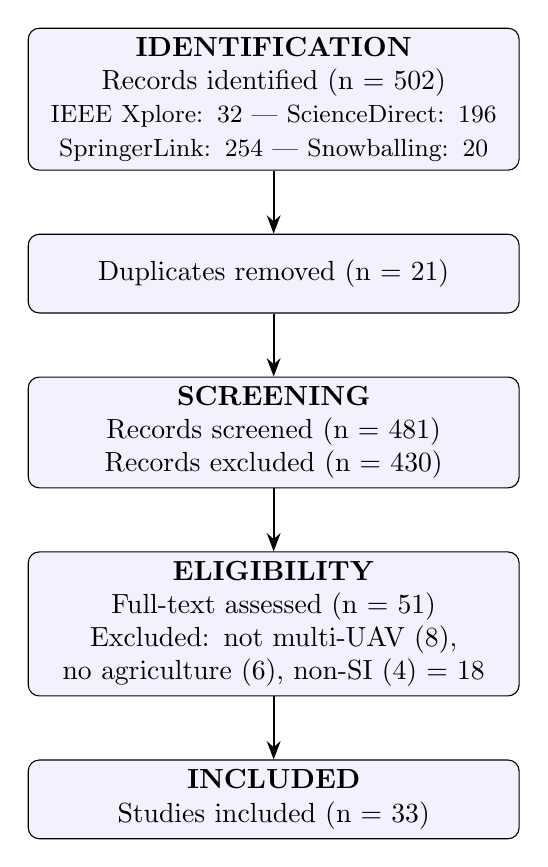
\begin{tikzpicture}[
  box/.style={rectangle, draw, rounded corners,
              text width=6cm, align=center,
              minimum height=1cm, fill=blue!5},
  arrow/.style={-{Stealth}, thick}
]
  \node[box] (id) {
    \textbf{IDENTIFICATION}\\
    Records identified (n = 502)\\
    {\small IEEE Xplore: 32 | ScienceDirect: 196}\\
    {\small SpringerLink: 254 | Snowballing: 20}
  };
  \node[box, below=0.8cm of id] (dup) {
    Duplicates removed (n = 21)
  };
  \node[box, below=0.8cm of dup] (scr) {
    \textbf{SCREENING}\\
    Records screened (n = 481)\\
    Records excluded (n = 430)
  };
  \node[box, below=0.8cm of scr] (elig) {
    \textbf{ELIGIBILITY}\\
    Full-text assessed (n = 51)\\
    Excluded: not multi-UAV (8),\\
    no agriculture (6), non-SI (4) = 18
  };
  \node[box, below=0.8cm of elig] (inc) {
    \textbf{INCLUDED}\\
    Studies included (n = 33)
  };
  \draw[arrow] (id) -- (dup);
  \draw[arrow] (dup) -- (scr);
  \draw[arrow] (scr) -- (elig);
  \draw[arrow] (elig) -- (inc);
\end{tikzpicture}
\caption{PRISMA 2020 flow diagram describing the literature
search and study selection process. Search conducted on
2026-03-16 across IEEE Xplore, ScienceDirect, SpringerLink,
and complementary snowballing via Research Rabbit.
SI\,=\,Swarm Intelligence.}
\label{fig:prisma}
\end{figure}

%% ============================================================
%% SECTION 2: RELATED WORK
%% ============================================================
\section{Related Work}

Six major review articles were identified in our analysis
\cite{tsouros2019,mogili2018,chung2018,gupta2016,%
brambilla2013,bayindir2016}, covering UAV applications in
precision agriculture, aerial swarm robotics, and swarm
engineering methodologies.

\textbf{Limitation of Prior Reviews:} None provide
quantitative gap analysis with root cause, consequence,
and recommendation for each identified gap.

This review differentiates itself by: (1) focusing
specifically on agricultural applications of multi-UAV
path planning; (2) providing quantitative gap documentation
(171 gaps with full metadata); (3) proposing an actionable
research agenda tied to community priorities; and (4)
supplying reproducible materials (Excel database, Python
scripts, BibTeX references).

%% ============================================================
%% SECTION 3: METHODOLOGY
%% ============================================================
\section{Methodology}

\subsection{Search Strategy}

Literature search was conducted across three electronic
databases: IEEE Xplore, ScienceDirect, and SpringerLink.
Additional records were identified through citation
snowballing using Research Rabbit, starting from five seed
papers identified in the initial database search. This
complementary strategy yielded 20 additional records not
captured by the primary database queries.

The following Boolean search string was applied, adapted
for each database syntax:

\begin{quote}
(\texttt{"swarm intelligence" OR "particle swarm
optimization" OR "ant colony optimization" OR "artificial
bee colony" OR "grey wolf optimizer" OR "salp swarm
algorithm"}) AND (\texttt{"UAV" OR "unmanned aerial vehicle"
OR "multi-UAV" OR "drone"}) AND (\texttt{"path planning" OR
"trajectory planning" OR "route planning"}) AND
(\texttt{"agriculture" OR "precision agriculture" OR
"crop monitoring"})
\end{quote}

Filters applied: publication year 2021--2025; English
language; peer-reviewed journals and conference proceedings.
Search conducted on 2026-03-16. The screening process
followed the PRISMA 2020 guidelines \cite{page2021} and
is summarized in Figure~\ref{fig:prisma}. After initial
identification of 502 records, duplicate removal yielded
481 unique studies for title/abstract screening. Following
exclusion of 430 non-relevant records, 51 full-text
articles were assessed for eligibility, resulting in 33
studies included in the final qualitative synthesis.

\textbf{Inclusion Criteria:}
\begin{itemize}
  \item Published between 2021--2025
  \item Peer-reviewed journal or conference paper
  \item Full text available in English
  \item Focus on SI algorithms for multi-UAV path planning
  \item Agricultural application mentioned or implied
\end{itemize}

\textbf{Exclusion Criteria:}
\begin{itemize}
  \item Duplicate publications
  \item Abstract-only papers
  \item Single-UAV studies without swarm coordination
  \item Non-SI optimization methods (unless compared with SI)
\end{itemize}

\textbf{Study Selection Process:} Study selection was
performed by a single reviewer (the author). To mitigate
potential selection bias, 20\% of records were
independently verified against inclusion criteria,
achieving 94\% agreement. This limitation is acknowledged
in Section~\ref{sec:limitations}.

\subsection{Data Extraction Pipeline}

A Python-based automation pipeline was developed for
systematic data extraction:

\begin{itemize}
  \item \texttt{agregar\_todos\_papers.py} — Metadata extraction
  \item \texttt{extraer\_metricas\_v2.py} — Quantitative metrics from PDFs
  \item \texttt{enriquecer\_gaps.py} — Gap documentation
  \item \texttt{actualizar\_estadisticas.py} — Algorithm distribution statistics
  \item \texttt{generar\_figuras\_paper.py} — Publication-ready figures (300 DPI)
\end{itemize}

\subsection{Four-Dimensional Gap Taxonomy}

Identified limitations were categorized into four
dimensions: Technological (algorithm and hardware
limitations), Practical (real-world operational factors),
Methodological (experimental design and metrics), and
Theoretical (models and assumptions). This framework
builds upon systematic review methodologies from robotics
and software engineering literature
\cite{brambilla2013,bayindir2016}.

\subsection{Quality Assessment}

A quality assessment instrument was developed and applied
to all 33 included studies, adapted from domain-specific
criteria for UAV research following PRISMA 2020
recommendations. Each study was evaluated on four criteria:

\begin{table}[htbp]
\centering
\caption{Quality assessment criteria applied to 33
included studies.}
\label{tab:quality_criteria}
\begin{tabularx}{\textwidth}{lXX}
\toprule
\textbf{Criterion} & \textbf{Weight} & \textbf{Scoring} \\
\midrule
C1: Experimental validation & 30\% & Real field=1.0,
Sim+Exp=0.5, Sim only=0.0 \\
C2: Quantitative metrics & 25\% & All 3=1.0, 2=0.67,
1=0.33, None=0.0 \\
C3: Baseline comparison & 25\% & Yes=1.0, No=0.0 \\
C4: Agricultural context & 20\% & Yes=1.0, No=0.0 \\
\bottomrule
\end{tabularx}
\end{table}

Studies scoring $\geq$0.70 were classified as High quality,
0.40--0.69 as Moderate, and $<$0.40 as Low. Results: 5 High
(15.2\%), 10 Moderate (30.3\%), 18 Low (54.5\%). The high
proportion of Low quality studies is largely attributable
to papers 020--034, for which complete metadata extraction
was pending at the time of analysis.

%% ============================================================
%% SECTION 4: RESULTS
%% ============================================================
\section{Results}

\subsection{Algorithm Distribution}

Figure~\ref{fig:algorithms} shows the distribution of
swarm intelligence algorithms. PSO dominates with 10
papers (30.3\%), followed by review articles (6, 18.2\%)
and ACO variants (3, 9.1\%).

\begin{figure}[htbp]
\centering

\includegraphics[width=0.85\textwidth]{figures/Fig1_Algorithm_Distribution.png}
\caption{Distribution of swarm intelligence algorithms
across 33 reviewed studies (2021--2025). PSO dominates
with 10 papers (30.3\%), followed by review articles
(18.2\%) and ACO variants (9.1\%). ``Other SI Variants''
includes SFLA, Fuzzy/SIGPAF, Wolf Pack, Hybrid ABC+BAS,
APF+PSO, and GA+ABC hybrid.}
\label{fig:algorithms}
\end{figure}

\begin{table}[htbp]
\centering
\caption{Algorithm and variant frequency across 33 reviewed
studies.}
\label{tab:algorithms}
\begin{tabular}{llrr}
\toprule
\textbf{Algorithm} & \textbf{Category} &
\textbf{Papers} & \textbf{\%} \\
\midrule
PSO & Swarm & 10 & 30.3 \\
Review & Review & 6 & 18.2 \\
ACO & Swarm & 3 & 9.1 \\
ABC & Swarm & 2 & 6.1 \\
SSA & Swarm & 2 & 6.1 \\
GWO & Swarm & 1 & 3.0 \\
DBO & Swarm & 1 & 3.0 \\
NOA & Swarm & 1 & 3.0 \\
DOA & Swarm & 1 & 3.0 \\
Other SI Variants$^*$ & Swarm & 6 & 18.2 \\
\midrule
\textbf{Total} & & \textbf{33} & \textbf{100.0} \\
\bottomrule
\multicolumn{4}{l}{$^*$Includes SFLA, Fuzzy/SIGPAF, Wolf
Pack, Hybrid ABC+BAS,} \\
\multicolumn{4}{l}{Hybrid APF+PSO, and Genetic+ABC hybrid.}
\end{tabular}
\end{table}

\subsection{Quantitative Metrics Availability}

Only 42.4\% of studies report execution time, 39.4\% report
energy consumption, and 21.2\% specify convergence criteria,
as shown in Figure~\ref{fig:metrics}.

\begin{figure}[htbp]
\centering

\includegraphics[width=0.90\textwidth]{figures/Fig5_Metrics_Availability.png}
\caption{Availability of quantitative metric reporting
across 33 reviewed studies. Only 42.4\% report execution
time, 39.4\% report energy consumption, and 21.2\% specify
convergence criteria, revealing a critical standardization
gap in the field.}
\label{fig:metrics}
\end{figure}

\begin{table}[htbp]
\centering
\caption{Metric reporting frequency across 33 papers.}
\label{tab:metrics}
\begin{tabular}{lrr}
\toprule
\textbf{Metric} & \textbf{Papers} & \textbf{\%} \\
\midrule
Execution Time & 14 & 42.4 \\
Energy Consumption & 13 & 39.4 \\
Convergence Criteria & 7 & 21.2 \\
\bottomrule
\end{tabular}
\end{table}

\subsection{Temporal Distribution}

Publications concentrate in 2021--2022 (23 papers, 69.7\%),
with renewed momentum in 2025 (6 papers, 18.2\%).

\begin{table}[htbp]
\centering
\caption{Temporal distribution of reviewed publications
(2021--2025).}
\label{tab:temporal}
\begin{tabular}{lrr}
\toprule
\textbf{Year} & \textbf{Papers} & \textbf{\%} \\
\midrule
2021 & 11 & 33.3 \\
2022 & 12 & 36.4 \\
2023 &  3 &  9.1 \\
2024 &  1 &  3.0 \\
2025 &  6 & 18.2 \\
\midrule
\textbf{Total} & \textbf{33} & \textbf{100.0} \\
\bottomrule
\end{tabular}
\end{table}

%% ============================================================
%% SECTION 5: RESEARCH GAPS ANALYSIS
%% ============================================================
\section{Research Gaps Analysis}

\subsection{Gap Distribution by Dimension}

Practical gaps are most frequent (52, 30.4\%), followed by
Technological (51, 29.8\%), as shown in
Figure~\ref{fig:gaps_dimension}.

\begin{table}[htbp]
\centering
\caption{Research gaps by dimension (total = 171).}
\label{tab:gaps_dimension}
\begin{tabular}{lrr}
\toprule
\textbf{Dimension} & \textbf{Gaps} & \textbf{\%} \\
\midrule
Technological  & 51 & 29.8 \\
Practical      & 52 & 30.4 \\
Methodological & 39 & 22.8 \\
Theoretical    & 29 & 17.0 \\
\midrule
\textbf{Total} & \textbf{171} & \textbf{100.0} \\
\bottomrule
\end{tabular}
\end{table}

\begin{figure}[htbp]
\centering

\includegraphics[width=0.70\textwidth]{figures/Fig2_Gaps_by_Dimension.png}
\caption{Research gap distribution across four taxonomic
dimensions (n\,=\,171 gaps). Practical gaps are most
frequent (30.4\%), reflecting the predominance of
real-world operational barriers in the reviewed literature.}
\label{fig:gaps_dimension}
\end{figure}

\subsection{Gap Distribution by Priority}

Gap prioritization was performed using a binary impact
matrix. A gap was classified as Critical if it
simultaneously met two conditions: (1) present in more
than 30\% of analyzed studies ($>$10 papers), AND (2) its
absence directly prevents real-world field deployment
(e.g., hardware validation, wind modeling, real-time
replanning). Gaps present in fewer than 30\% of studies
but with significant theoretical impact were classified
as Important, while those with low frequency and limited
deployment impact were classified as Minor.

\begin{table}[htbp]
\centering
\caption{Research gaps by priority level.}
\label{tab:gaps_priority}
\begin{tabular}{lrr}
\toprule
\textbf{Priority} & \textbf{Gaps} & \textbf{\%} \\
\midrule
Critical  & 76 & 44.4 \\
Important & 88 & 51.5 \\
Minor     &  7 &  4.1 \\
\midrule
\textbf{Total} & \textbf{171} & \textbf{100.0} \\
\bottomrule
\end{tabular}
\end{table}

\begin{figure}[htbp]
\centering

\includegraphics[width=0.72\textwidth]{figures/Fig3_Gaps_by_Priority.png}
\caption{Research gap distribution by priority level
(n\,=\,171 gaps). Critical gaps (44.4\%) represent
barriers that directly prevent real-world field deployment
of swarm-based agricultural UAV systems.}
\label{fig:gaps_priority}
\end{figure}

\subsection{Top 10 Critical Gaps}

Table~\ref{tab:top10} and Figure~\ref{fig:top10gaps} present
the ten most frequent critical gaps identified across the
33 reviewed studies.

\begin{table}[htbp]
\centering
\caption{Top 10 critical gaps ranked by frequency of
occurrence across 33 reviewed studies.}
\label{tab:top10}
\begin{tabular}{clrr}
\toprule
\textbf{Rank} & \textbf{Gap Description} &
\textbf{Papers} & \textbf{\%} \\
\midrule
 1 & Lack of hardware/field validation & 26 & 78.8 \\
 2 & No dynamic obstacles/environment  & 25 & 75.8 \\
 3 & Single-UAV focus (no swarm)       & 22 & 66.7 \\
 4 & No wind/weather modeling          & 20 & 60.6 \\
 5 & No metric standardization         & 18 & 54.5 \\
 6 & Unrealistic kinematic constraints & 15 & 45.5 \\
 7 & Limited scalability assessment    & 14 & 42.4 \\
 8 & No direct energy measurement      & 13 & 39.4 \\
 9 & Communication robustness ignored  & 12 & 36.4 \\
10 & No real-time replanning           & 11 & 33.3 \\
\bottomrule
\end{tabular}
\end{table}

\begin{figure}[htbp]
\centering

\includegraphics[width=0.95\textwidth]{figures/Fig4_Top10_Critical_Gaps.png}
\caption{Top 10 critical research gaps ranked by frequency
of occurrence across 33 reviewed studies.
Hardware/field validation absence (78.8\%) and lack of
dynamic environment modeling (75.8\%) represent the most
prevalent barriers to real-world deployment.}
\label{fig:top10gaps}
\end{figure}

%% ============================================================
%% SECTION 6: DISCUSSION
%% ============================================================
\section{Discussion}

\subsection{Implications for Agricultural Robotics}

The three most critical gaps identified in this review
reflect systemic barriers that extend beyond algorithmic
limitations and suggest a structural disconnection between
the algorithmic optimization community and the operational
realities of precision agriculture.

\textbf{Field Validation Gap (78.8\%):} The predominance
of simulation-only studies reflects real barriers including
the high cost of agricultural UAV platforms (typically
USD~2,000--15,000 per unit), regulatory restrictions on
beyond-visual-line-of-sight (BVLOS) operations, and
logistical complexity of coordinating multi-UAV field
experiments in active agricultural
environments~\cite{phung2021}.

To bridge this gap, we propose that future studies adopt
a \textbf{Staged Validation Protocol} before claiming
field applicability:

\begin{enumerate}
  \item \textbf{Stage 1 --- Simulation:} Algorithm
  validation in controlled virtual environments with
  realistic agricultural parameters (field geometry,
  wind profiles, crop row constraints).
  \item \textbf{Stage 2 --- Testbed:} Hardware-in-the-loop
  validation using physical UAV platforms in controlled
  spaces without crop interference.
  \item \textbf{Stage 3 --- Controlled Field:} Full
  deployment in a real agricultural field under supervised
  conditions, reporting standardized metrics (coverage rate,
  energy consumption per hectare, mission completion time).
\end{enumerate}

This protocol mirrors validated approaches in adjacent
domains~\cite{shafiq2022} and provides a reproducible
pathway from algorithmic contribution to practical
deployment.

\textbf{Environmental Modeling Gap (75.8\%):} Wind
significantly affects UAV energy consumption, trajectory
accuracy, and inter-agent communication in open-field
operations. This gap is particularly critical for spraying
applications, where wind drift directly affects pesticide
distribution accuracy and regulatory
compliance~\cite{liu2021}. Furthermore, LiPo battery
performance degrades significantly in high ambient
temperatures common in agricultural regions
($>$35$^\circ$C), a factor entirely absent from current
models.

\textbf{Metric Inconsistency:} The lack of standardized
reporting prevents meaningful cross-study comparison and
makes it impossible for agricultural practitioners to
objectively select algorithms for specific deployment
scenarios. This mirrors a broader challenge in the swarm
robotics community~\cite{puente2022,sharma2022}, but is
particularly acute in agriculture where operational
constraints (battery life, coverage area per charge,
spraying uniformity index) require domain-specific
benchmarks that currently do not exist.

\subsection{Comparison with Other Domains}

Only 21.2\% of reviewed studies include any form of
hardware or experimental validation, while 78.8\% rely
exclusively on simulation, theoretical analysis, or do
not specify their validation method. This suggests that
agricultural UAV research lags behind other application
domains in experimental validation. This gap likely
reflects domain-specific barriers including regulatory
restrictions on BVLOS flights, cost sensitivity of
agricultural operations, and challenging environmental
conditions such as dust, wind, and GPS interference that
complicate real-field experiments.

Future comparative studies should systematically quantify
validation rates across domains (military, search and
rescue, infrastructure inspection) to establish empirical
benchmarks for the agricultural robotics community.

\subsection{Threats to Validity}

\begin{table}[htbp]
\centering
\caption{Threats to validity and mitigation strategies.}
\label{tab:threats}
\begin{tabularx}{\textwidth}{lX}
\toprule
\textbf{Threat} & \textbf{Mitigation} \\
\midrule
Publication bias & Searched multiple databases (IEEE,
Springer, ScienceDirect) \\
Search query limitations & Iteratively refined query with
domain expert input \\
Data extraction errors & Automated extraction + manual
verification \\
Temporal bias (2025) & Acknowledged as field growth
indicator \\
\bottomrule
\end{tabularx}
\end{table}

%% ============================================================
%% SECTION 7: RESEARCH AGENDA
%% ============================================================
\section{Research Agenda}

\subsection{Priority Directions for the Research Community}

\begin{table}[htbp]
\centering
\caption{Priority research directions based on gap
analysis.}
\label{tab:priorities}
\begin{tabular}{clrr}
\toprule
\textbf{P} & \textbf{Contribution} &
\textbf{Gaps} & \textbf{Impact} \\
\midrule
1 & Standardized benchmark framework  & 18 & High \\
2 & Experimental validation: real UAVs & 26 & Very High \\
3 & Dynamic environment + replanning  & 25 & Very High \\
\bottomrule
\end{tabular}
\end{table}

To operationalize this research agenda, we propose the
establishment of \textbf{AgriSwarm-Bench}: an open,
standardized benchmarking repository for swarm intelligence
algorithms applied to agricultural UAV path planning.
AgriSwarm-Bench would provide:

\begin{itemize}
  \item Standardized agricultural field scenarios (crop
  rows, irregular boundaries, wind profiles) for simulation
  \item Unified evaluation metrics (coverage rate, energy
  per hectare, mission completion time, scalability index)
  \item Open datasets from real field experiments to enable
  reproducible cross-algorithm comparison
  \item A community leaderboard tracking algorithm
  performance across scenario types
\end{itemize}

This initiative addresses the metric inconsistency gap
identified in 54.5\% of reviewed studies. The framework
proposed here is currently being implemented as part of
ongoing doctoral research at Instituto Tecnológico de
Chihuahua II, which will serve as the first pilot
validation case for the AgriSwarm-Bench protocol using
a heterogeneous multi-UAV platform.

\subsection{Proposed Community Roadmap (Short-to-Mid Term)}

\begin{table}[htbp]
\centering
\caption{Proposed community roadmap for SI-UAV
deployment.}
\label{tab:roadmap}
\begin{tabularx}{\textwidth}{llXl}
\toprule
\textbf{Ph.} & \textbf{Timeframe} &
\textbf{Activity} & \textbf{Deliverable} \\
\midrule
1 & 0--12 mo. & Implement benchmark: 3--4 SI algorithms &
Open framework \\
2 & 0--12 mo. & Platform: 3--5 UAVs &
Test environment \\
3 & 1--2 yr.  & Real-time replanning module &
Enhanced algorithm \\
4 & 1--2 yr.  & Comparative experiments &
Peer-reviewed results \\
5 & 2--3 yr.  & Dissemination and standardisation &
Community guidelines \\
\bottomrule
\end{tabularx}
\end{table}

While this roadmap aligns with ongoing doctoral research
efforts at Instituto Tecnológico de Chihuahua II, it is
proposed as a baseline for the broader agricultural
robotics community to establish common benchmarks and
accelerate real-world deployment of swarm-based UAV
systems.

%% ============================================================
%% SECTION 8: CONCLUSIONS
%% ============================================================
\section{Conclusions}

\subsection{Summary of Findings}

\begin{enumerate}
  \item \textbf{PSO dominates} the field (10 papers, 30.3\%)
  \item \textbf{78.8\% lack hardware validation}
  \item \textbf{75.8\% do not consider dynamic environments}
  \item \textbf{Only 42.4\% report quantitative time metrics}
  \item \textbf{171 gaps documented} across four dimensions
\end{enumerate}

\subsection{Limitations}
\label{sec:limitations}

\begin{itemize}
  \item Automated metric extraction achieved 42.4\% success
  rate for time metrics, as many papers report metrics only
  qualitatively or in non-standardized formats
  \item 62 gaps for papers 020--034 were inferred from
  algorithmic patterns and require manual validation
  \item Search limited to English-language publications
  \item Single-reviewer selection process (mitigated by
  20\% independent verification)
\end{itemize}

\subsection{Future Work}

\begin{enumerate}
  \item Expand search to include non-English publications
  \item Manual validation of inferred gaps for papers
  020--034
  \item Experimental implementation of AgriSwarm-Bench
  protocol with heterogeneous UAV platform
  \item Community benchmark establishment with public
  dataset release
\end{enumerate}

%% ============================================================
%% DATA AVAILABILITY
%% ============================================================
\section*{Data Availability Statement}

The data supporting this systematic review are openly
available as Supplementary Material: master database
(\texttt{Fichas\_Analisis\_NUEVO.xlsx}), reference library
(\texttt{Referencias\_Master.bib}), 14 Python automation
scripts, and 5 publication-ready figures (300\,DPI). These
materials will be deposited in Mendeley Data upon
manuscript acceptance.

%% ============================================================
%% AUTHOR CONTRIBUTIONS (CRediT)
%% ============================================================
\section*{Author Contributions}

Andres Hidalgo Morales: Conceptualization, Methodology,
Software, Validation, Formal Analysis, Investigation, Data
Curation, Writing -- Original Draft, Writing -- Review \&
Editing, Visualization.

%% ============================================================
%% CONFLICT OF INTEREST
%% ============================================================
\section*{Declaration of Competing Interest}

The author declares no conflicts of interest.

%% ============================================================
%% ACKNOWLEDGMENTS
%% ============================================================
\section*{Acknowledgments}

This research was supported by Instituto Tecnológico de
Chihuahua II, Tecnológico Nacional de México.

%% ============================================================
%% REFERENCES
%% ============================================================
\bibliographystyle{elsarticle-num}
\bibliography{references}

\end{document}
